\documentclass[12pt,a4paper]{article}
\usepackage[UTF8]{ctex}
\usepackage[backend=biber]{biblatex}
\addbibresource{references.bib}
\usepackage{amsmath,amsthm,amssymb,graphicx,multirow,float,caption}
\usepackage{geometry}
\geometry{left=2.54cm, right=2.54cm, top=3.18cm, bottom=3.18cm}
\usepackage{enumitem}
\usepackage{subcaption,booktabs,diagbox}
\setenumerate[1]{itemsep=0pt,partopsep=0pt,parsep=\parskip,topsep=5pt}
\setitemize[1]{itemsep=0pt,partopsep=0pt,parsep=\parskip,topsep=5pt}
\setdescription{itemsep=0pt,partopsep=0pt,parsep=\parskip,topsep=5pt}
\usepackage{adjustbox}
\usepackage[graphicx]{realboxes}
\usepackage{rotating}

\usepackage{titlesec}

\newcommand{\be}[1]{
    \begin{equation}
        #1
    \end{equation}
}

\newcommand{\bfig}[3]{
    \begin{figure}[H]
        \centering
        \includegraphics[width=#1\textwidth]{#2}
        \caption{#3}
    \end{figure}
}

\titleformat{\section}%设置section的样式
{\raggedright\large\bfseries}%右对齐,4号字,加粗
{\thesection .\quad}%标号后面有个点
{0pt}%sep label和title之间的水平距离
{}%标题前没有内容

\title{\vspace{-4cm}\Large 连续与脉冲核磁共振}  %文章标题
\author{\kaishu 学号:202111030007 \hspace{2cm} 姓名:郑晓旸}   %作者的名称
\date{}

\begin{document}
\maketitle

\begin{abstract}
    本实验基于连续核磁共振谱仪和脉冲式核磁共振谱仪观测了 H 核的共振信号, 并在不同化学环境下测量了 H 核的弛豫时间等参数。
    首先, 利用连续核磁共振谱仪, 借助示波器测量得到了 5\%$CuS O_4$ 溶液的共振频率 $f = 21.4655 MHz$, 后对 PID 信号进行拟合尾波峰, 得到表观弛豫时间
    $T_2^{\star} = 0.5984ms$, 并据此计算了磁场不均匀度 $\frac{\Delta B}{B}= 61.1(ppm)$。
    后进一步测量不同浓度 $CuS O_4$ 溶液的共振信号强度和表观弛豫时间 $T_2^{\star}$, 观察不同浓度下的
    表观弛豫时间 $T_2^{\star}$, 分析得出结论 $CuS O_4$ 作为溶质质具有增强共振信号的作用。
    然后采用脉冲式核磁共振谱仪, 利用 FID 信号和自旋回波信号, 观测了不
    同浓度 $CuS O_4$ 溶液的表观弛豫时间 $T_2^{\star}$ 和本征弛豫时间 $T_2$。并绘制折线图, 得
    出结论 $T_2$ 和 $T_2^{\star}$ 随着浓度的增大而减小。
    最后测量了甘油和二甲苯的频谱, 和二甲苯的化学位移。 二甲苯化学位移$\delta =4.659ppm$, 有两种等效氢分别对应着苯环和甲基上的 H 原子。
\end{abstract}

\section{引言}
核磁共振技术(NMR)自 1945 年由 Felix Bloch 和 Edward Purcell 独立发明\cite{Bloch1946,Purcell1946}以来,已经成为现代科学研究中不可或缺的一种技术。它不仅大大提高了核磁矩测量的精度,还推动了物理学、化学、生物学和医学等多个学科的发展。本技术的核心在于利用外部磁场影响原子核的磁性,通过检测其响应来揭示物质的微观结构和动态行为。

在过去几十年中,NMR 技术经历了显著的进化,特别是在设备和应用方法上的创新\cite{Levitt2008}。这种技术现在已经拓展到了连续波谱仪和脉冲波谱仪两种主要形式。连续波谱仪通过不断施加射频场来获取频率谱,而脉冲波谱仪则利用短暂的射频脉冲来产生时间谱,这些时间谱经过傅立叶变换后可以转换为频率谱。这些进展不仅提高了谱的分辨率,还增强了样品信息的提取能力,使得 NMR 成为了研究复杂化学和生物结构的强有力工具。

NMR 的非侵入性质使其特别适用于活体生物的研究,这一特点在医学领域尤为重要,特别是在核磁共振成像(MRI)技术中的应用\cite{Lauterbur1973}。它提供了一种强大的手段来检测和诊断各种疾病,而不对生物体造成伤害。

在本实验中,我们将以水中的氢核作为主要研究对象,通过使用连续波和脉冲波谱仪来探究核磁共振的基本原理及其观测方法。通过这些实验,我们旨在深入理解 NMR 技术的工作原理及其在科学研究中的广泛应用。
\section{计算公式}
\subsection{磁场不均匀度}
磁场不均匀度计算公式\cite{Ernst1987},
\be{\frac{\Delta B}{B_{0}}=\frac{2 \pi \omega_{m} \ln \left(y / y_{0}\right)}{\omega_{0} \arcsin \left(x / x_{0}\right)}}
其中,$\omega_m$,$\omega_0$  分别为磁场扫场和共振时的圆频率,$y$ 为某一峰的峰值,x 为最大峰至此峰的距离,$y_0$ 为共振峰
高, $x_{0}$为共振峰至尾波消失点距离。
\subsection{化学位移}
以参数 $\sigma$表示环境对磁场的屏蔽作用, 即原子感受到的磁场 $B=B_{0}(1-\sigma)$, 因此在不同的化学环境下
共振频率为$\omega_{0}=\gamma(1-\sigma) B_{0}$。

在外磁场 $B_0$ 不变的情况下, 依次测量参照物的共振频率 $\omega_s$ 及样品的共振频率 $\omega_R$, 定义相对化学位移
$\delta$ 为:
\be{\delta=\frac{\sigma_{R_{2}}-\sigma_{R_{1}}}{1-\sigma_{s}} \times 10^{6} \mathrm{ppm}=\frac{\omega_{R_{2}}-\omega_{R_{1}}}{\omega_{s}} \times 10^{6} \mathrm{ppm}}

\section{结果分析与讨论}
\subsection{连续核磁共振谱仪}
放入 5\% 浓度的 $CuS O_4$ 样品, 基于仪器上的参考位置及参考频率, 仔细调节至出现明显的共振信号,
得到的共振信号如下图所示:
\bfig{0.7}{pic.jpeg}{5\%$CuSO_4$溶液连续谱仪信号}
当$CuS O_4$浓度增大降低时,共振的弛豫时间增长,导致在两次发生核磁共振的时间间隔中为完全达到平衡状态,因此共振信号的形式会形成类似高斯波包的形式\cite{Fukushima1981}。如下图所示:
\bfig{0.7}{pic2.jpeg}{0.05\%$CuSO_4$溶液连续谱仪信号}
利用示波器光标测量同一周期内共振信号时间间隔, 测量得到样品的共振频率为 $f = 21.4655MHz$。

\subsubsection{表观弛豫时间测量}
调节出最优尾波信号后, 开始测量逐峰测量尾波强度. 各尾波峰值处的纵坐标呈指数衰减. 

依次测量各峰的位置及大小, 并采取指数函数$U=a \exp \left(-\frac{t}{T^{\star}}\right)+c$拟合得到曲线如下图所示:
\bfig{0.6}{5弛豫时间拟合.png}{5\% 样品溶液 $T_2^{\star}$ 拟合}
其中测量得到结果, 共振信号峰值 $U_M = 1.0652V$, 通过拟合得到表观弛豫时间 $T_2^{\star} = 0.5984ms$。

\subsubsection{不同浓度的 CuSO4 样品共振信号测量}
取出 5\%$CuS O_4$ 样品溶液, 在保证装置位置不变的情况下, 依次放入 1\%, 0.5\%, 0.05\%$CuS O_4$ 溶液及纯
水溶液。采取相同的方法读取尾波峰的大小和位置, 作拟合得到曲线如下图所示:

\begin{figure}[ht]
\centering
\begin{subfigure}[b]{0.45\textwidth}
    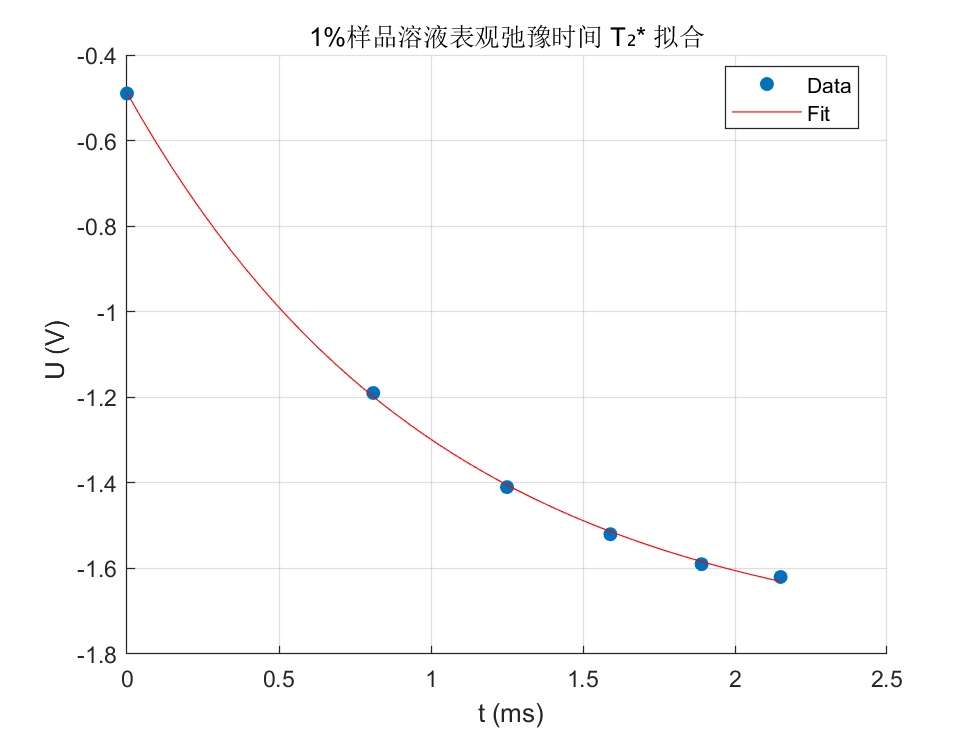
\includegraphics[width=\textwidth]{1弛豫时间拟合.png}
    \caption{1\%$CuSO_4$溶液连续谱仪信号}
\end{subfigure}
\hfill
\begin{subfigure}[b]{0.45\textwidth}
    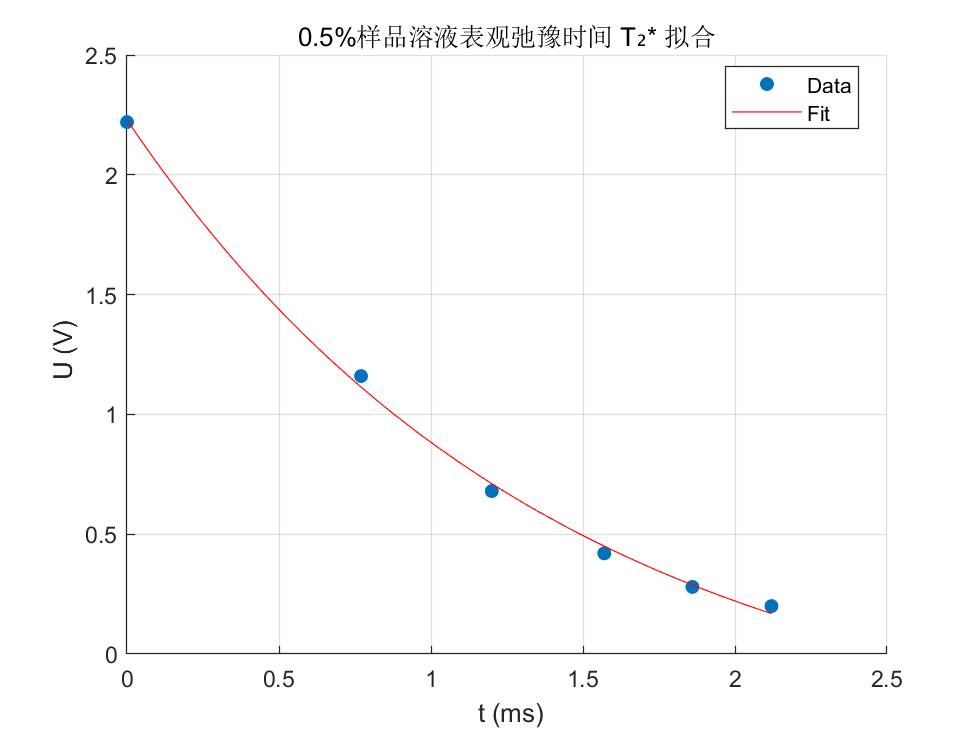
\includegraphics[width=\textwidth]{05弛豫时间拟合.png}
    \caption{0.5\%$CuSO_4$溶液连续谱仪信号}
\end{subfigure}

\begin{subfigure}[b]{0.45\textwidth}
    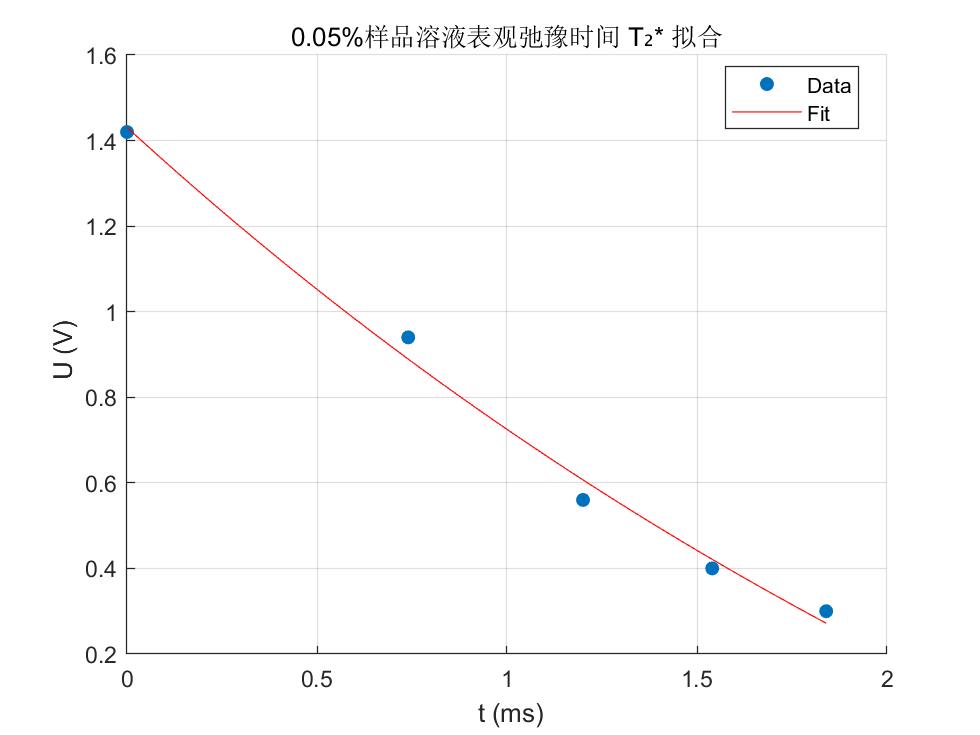
\includegraphics[width=\textwidth]{005弛豫时间拟合.png}
    \caption{0.05\%$CuSO_4$溶液连续谱仪信号}
\end{subfigure}
\hfill
\begin{subfigure}[b]{0.45\textwidth}
    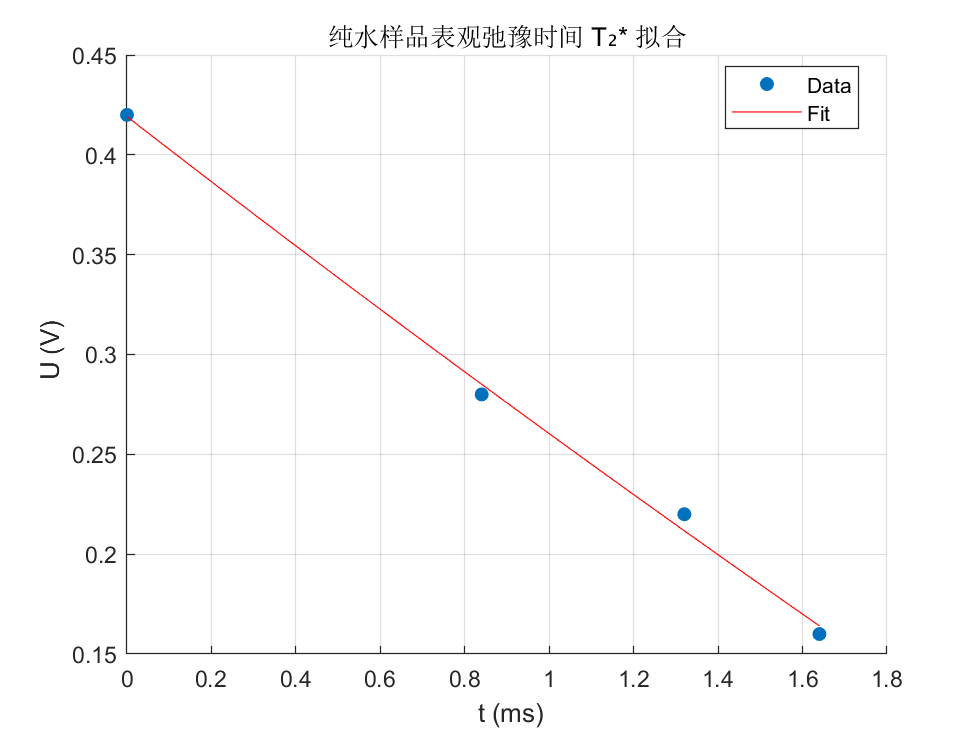
\includegraphics[width=\textwidth]{纯水弛豫时间拟合.png}
    \caption{纯水溶液连续谱仪信号}
\end{subfigure}
\end{figure}


拟合得到不同浓度溶液的表观弛豫时间 $T_2^{\star}$ 和最大振幅 $U_M$ 如下表所示:
\begin{table}[H]
    \centering
    \begin{tabular}{|c|c|c|c|c|c|}
    \hline
    浓度($\%$) & 0      & 0.05  & 0.5   & 1     & 5     \\ \hline
    $U_M(V)$     & 2.498  & 2.795 & 2.649 & 1.303 & 1.065 \\ \hline
   $T_2^{\star}(ms)$          & 15.227 & 3.436 & 1.411 & 1.029 & 0.598 \\ \hline
    \end{tabular}
    \caption{不同浓度样品结果表}
    \end{table}

    观察上表能得出结论, 表观弛豫时间与浓度呈现出现负相关性, 样品浓度越小, 表观弛豫时间越长, 表现为尾波的峰值曲线更贴近直线.

此外, 可以看出满足如下趋势, 随着 $CuS O_4$ 溶液浓度增大, 共振信号的峰值增大。原因可能是
由于 $Cu^{2+}$ 具有顺磁性, 可以增强 H 核的局域磁场的均匀度。因此 $CuS O_4$ 作为溶质可以提高共振信号的
强度, 增强信号信噪比, 使信号更加明显。

\subsubsection{磁场不均匀度测量}
依据磁场不均匀度计算公式, 
\be{\frac{\Delta B}{B_{0}}=\frac{2 \pi \omega_{m} \ln \left(y_{0} / y\right)}{\omega_{0} \arcsin \left(x / x_{0}\right)}}
选取信号效果较好的 5\%$CuS O_4$ 溶液, 根据前文测量得到物理量, 尾波峰高$y=0.0653V$, 共振峰高 $y_0 = 1.0629V$, 共振峰至尾
波消失点距离 $x_0 = 2.68ms$, 共振峰至尾波峰位距离$x=1.66ms$将数据 (已将时间零点移动至第一个共振峰的位置) 代入计算公式得到不均匀
度得到

\be{\frac{\Delta B}{B}=\frac{2\pi\times 50Hz\times ln(\frac{1.0629}{0.0653})}{21.4655MHz\times \arcsin{\frac{1.66}{2.68}}}=61.1ppm}

\subsection{脉冲核磁共振谱仪}
\subsubsection{0.05\%$CuSO_4$ 溶液弛豫时间测量}
选择 0.05\%$CuS O_4$ 溶液, 打开 PNMR 软件调节脉冲参数, 观察到 FID 信号及自旋回波信号, 调节调场及
扫场旋钮至信号最优, 进行弛豫时间的测量。利用软件的采样及拟合部分, 测量示意图如下:


\begin{figure}[ht]
\centering
\begin{subfigure}[b]{0.45\textwidth}
    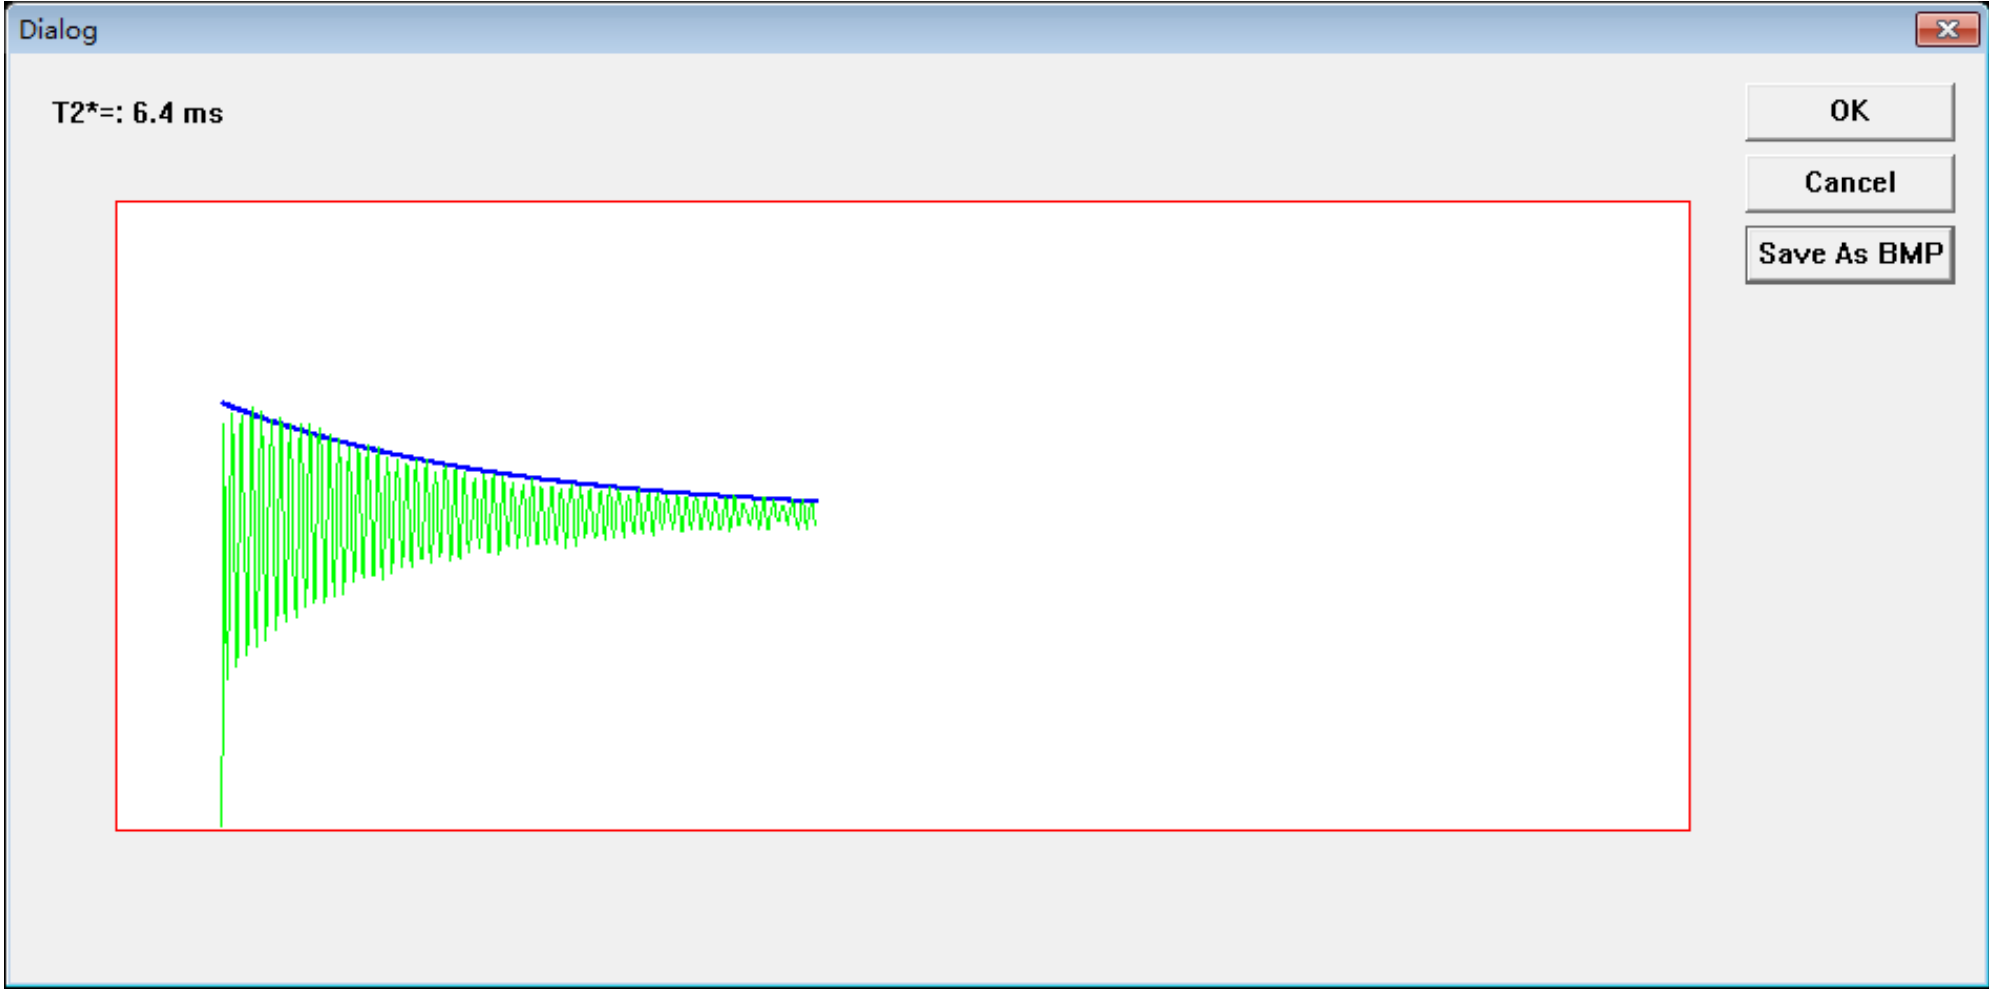
\includegraphics[width=\textwidth]{脉冲表观弛豫时间.png}
    \caption{表观弛豫时间$T_2^{\star}$测量}
\end{subfigure}
\hfill % 保持图片之间的间距
\begin{subfigure}[b]{0.45\textwidth}
    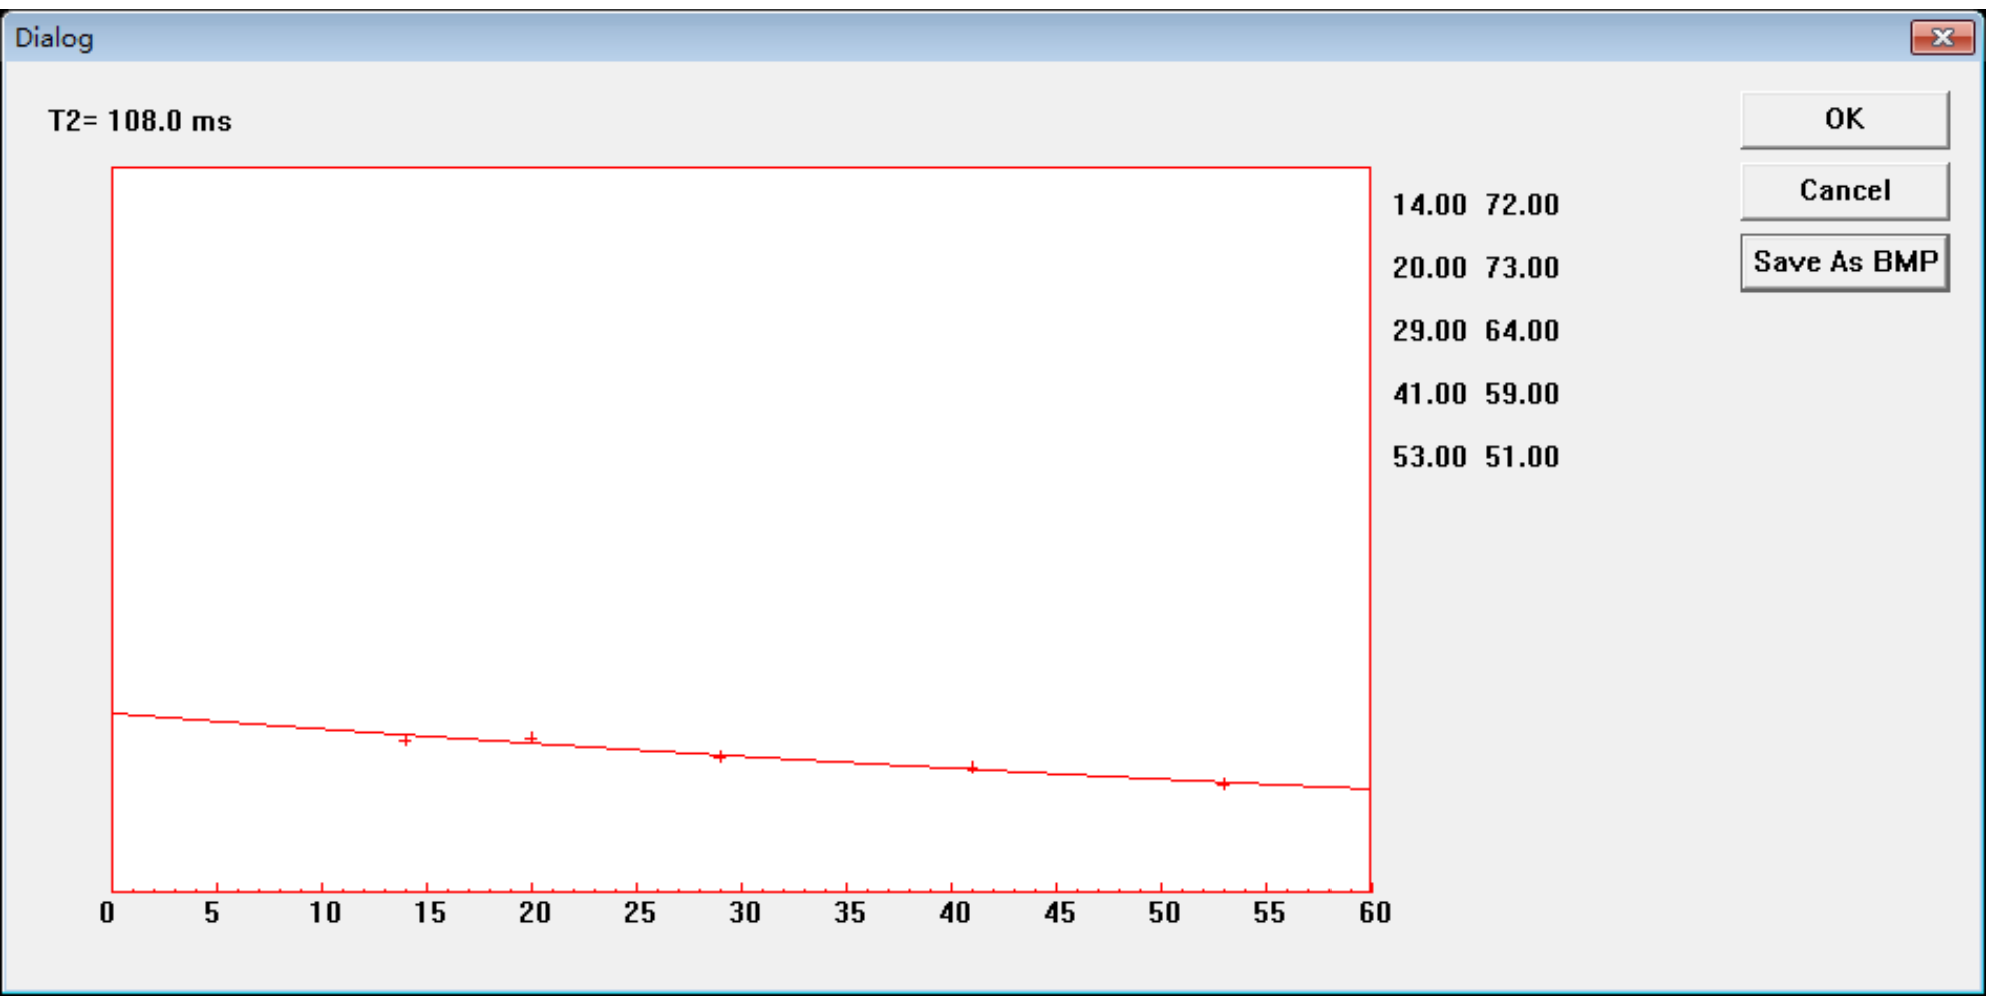
\includegraphics[width=\textwidth]{脉冲弛豫时间.png}
    \caption{本征弛豫时间$T_2$测量}
\end{subfigure}

\end{figure}




\begin{itemize}
    \item \textbf{表观横向弛豫时间 $T_2^{\star}$}

    测得0.5\%$CuS O_4$ 溶液表观弛豫时间 $T_2^{\star} = 6.1ms$。

    \item \textbf{本征横向弛豫时间 $T_2$}
    
    测得0.5\%$CuS O_4$ 溶液本征弛豫时间 $T_2 = 147.5ms$。
\end{itemize}

\subsubsection{不同浓度弛豫时间测量}
取出 0.05\%$CuS O_4$ 溶液, 依次放入0.5\%, 1\%, 5\% 浓度的样品溶液, 利用 FID 信号及自旋回波信号
依次测量表观弛豫时间和本征弛豫时间, 重复取样三次得到结果如下表所示:
\begin{table}[H]
    \centering 
    \begin{tabular}{|c|c|c|c|c|}
    \hline
    浓度($\%$)  & 0.05  & 0.5  & 1    & 5   \\ \hline
    $T_2^{\star}(ms)$ & 6.1   & 4.6  & 6    & 2.4 \\ \hline
    $T_2(ms)$  & 147.5 & 25.5 & 13.3 &     \\ \hline
    \end{tabular}
    \caption{不同浓度弛豫时间测量结果表}
    \end{table}

其中 5\% 样品溶液未观测到自旋回波信号, 无法拟合测量本征弛豫时间。

观察发现本征弛豫时间 $T_2$ 与浓度呈现出负相关。推测 5\% 浓度对应的本征弛豫时间相对较小, 自旋
回波信号的幅值更小, 因此在实验中难以观察到 5\% 浓度的自旋回波信号,与实验现象相符.

\subsection{化学位移}
\begin{itemize}
    \item \textbf{甘油}
    
    调节脉冲 FID 信号幅值最大后, 取出 $CuS O_4$ 样品, 放入甘油样品, 单次测量并进行频域分析, 得到结
果如下图所示:
\bfig{0.7}{甘油.png}{甘油 FID 频域信号}

读出甘油的共振频率 $f_R = 4658Hz$, 仅有一个共振频率, 无化学位移, 反映了甘油中 C − H 中的 H 核化
学环境大致相同。

    \item \textbf{二甲苯}
    
    取出甘油样品, 放入二甲苯样品, 单次测量并进行频域分析, 得到结果如下图所示:

    \bfig{0.7}{二甲苯.png}{二甲苯 FID 频域信号}

    读出二甲苯的两个共振频率 $f_{R1} = 4607Hz$, $f_{R2} = 4707Hz$, 计算得到化学位移:

    \be{\delta= 4.659\mathrm{ppm}}
    可明显观察到两个共振频率, 说明二甲苯中存在两种不同环境的 H 核, 分别对应着苯环和甲基上的 H
原子。
\end{itemize}

\section{结论}
本实验基于连续核磁共振谱仪和脉冲式核磁共振谱仪观测了 H 核的共振信号, 并在不同化学环境下测量了 H 核的弛豫时间等参数。
首先, 利用连续核磁共振谱仪, 借助示波器测量得到了 5\%$CuS O_4$ 溶液的共振频率 $f = 21.4655 MHz$, 后对 PID 信号进行拟合尾波峰, 得到表观弛豫时间
$T_2^{\star} = 0.5984ms$, 并据此计算了磁场不均匀度 $\frac{\Delta B}{B}= 61.1(ppm)$。
后进一步测量不同浓度 $CuS O_4$ 溶液的共振信号强度和表观弛豫时间 $T_2^{\star}$, 观察不同浓度下的
表观弛豫时间 $T_2^{\star}$, 分析得出结论 $CuS O_4$ 作为溶质质具有增强共振信号的作用。
然后采用脉冲式核磁共振谱仪, 利用 FID 信号和自旋回波信号, 观测了不
同浓度 $CuS O_4$ 溶液的表观弛豫时间 $T_2^{\star}$ 和本征弛豫时间 $T_2$。并绘制折线图, 得
出结论 $T_2$ 和 $T_2^{\star}$ 随着浓度的增大而减小。
最后测量了甘油和二甲苯的频谱, 和二甲苯的化学位移。 二甲苯化学位移$\delta =4.659ppm$, 有两种等效氢分别对应着苯环和甲基上的 H 原子。

\printbibliography
\newpage
\section{附录. 实验数据记录}
\begin{figure}[H]
    \centering
    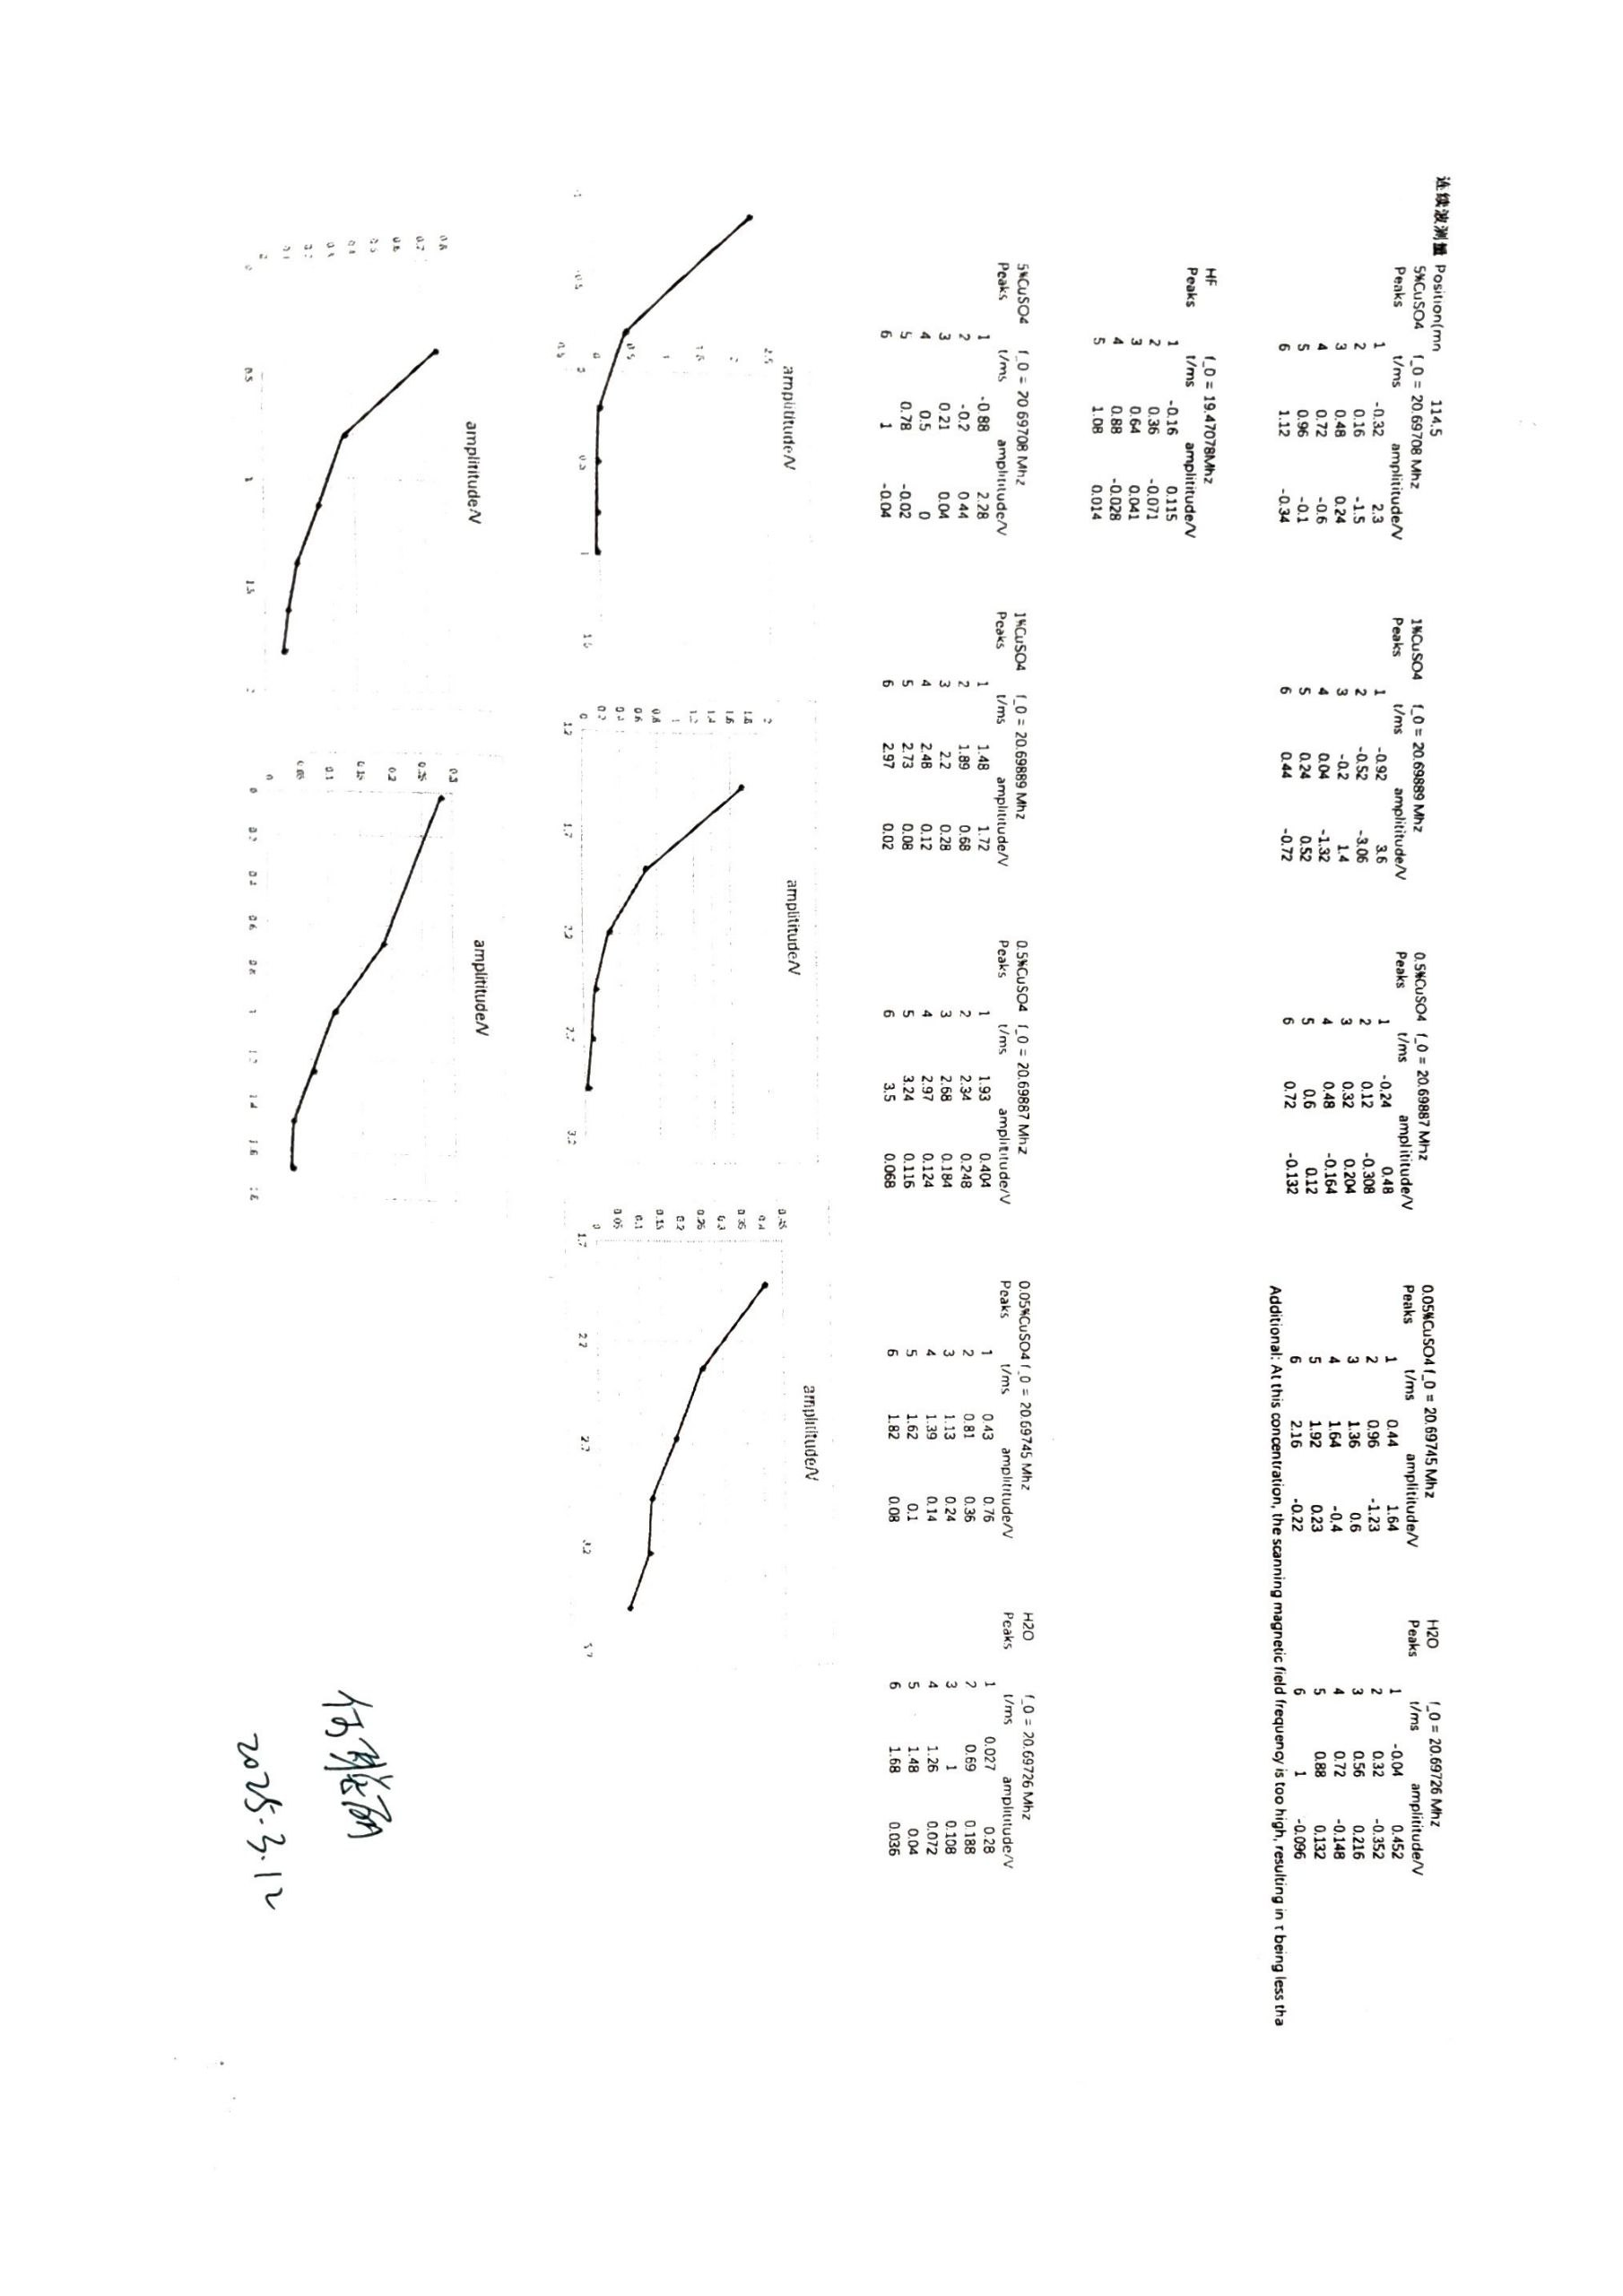
\includegraphics[width=\textwidth]{Raw.jpg}
    \caption{实验数据记录}
\end{figure}
\end{document}